\documentclass[10pt]{extarticle}
\usepackage[a4paper,margin=1.5cm,columnsep=0.7cm]{geometry}
\usepackage{amsmath,amssymb}
\usepackage{graphicx}
\usepackage{enumitem}
\usepackage{booktabs}
\usepackage{array}
\usepackage{tabularx}
\usepackage[T1]{fontenc}
\usepackage{multicol}

\setlength{\parindent}{0pt}
\setlength{\parskip}{4pt}
\renewcommand{\arraystretch}{1.15}

\newenvironment{qoptions}{\begin{itemize}[leftmargin=1.8em,itemsep=2pt,topsep=2pt,label={}]}{\end{itemize}}
\newcommand{\opt}[2]{\item[({#1})] {#2}}

\newcommand{\sectionhdr}[1]{\par\vspace{4pt}\noindent\textbf{\large #1}\par\vspace{2pt}}
\newcommand{\subsectionhdr}[1]{\par\vspace{3pt}\noindent\textbf{#1}\par\vspace{2pt}}

\pagestyle{empty}

\begin{document}
\begin{center}
{\LARGE\bfseries JEE (Main+Advanced) Score-II --- Test 42 (19 Mar 2025)}
\end{center}
\vspace{6pt}

\begin{multicols}{2}

\sectionhdr{PART-1: PHYSICS}
\subsectionhdr{Section-I: One or more correct}

\textbf{1.} A system of three small spheres, each with mass m, connected by inextensible wires of negligible mass into the shape of a horizontal equilateral triangle with side length $\ell$ (see Fig.), slides without friction on a horizontal icy surface. At a certain moment, sphere A is moving with velocity v in the direction of AB, and the instantaneous velocity of sphere B is parallel to line BC.

\begin{center}
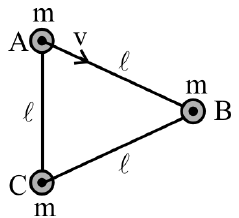
\includegraphics[width=0.55\linewidth]{Score-II - Test 42 (19 Mar 2025)-img/p1phy_q1_triangle.png}
\end{center}

\begin{qoptions}
\opt{A}{The instantaneous speed of B is $v\sqrt5$.}
\opt{B}{The angular velocity of the system is $\dfrac v{2\ell}$.}
\opt{C}{The magnitude of force acting on the wires connecting the spheres is $\dfrac{2mv^2}\ell$.}
\opt{D}{None of the above}
\end{qoptions}

\textbf{2.} Consider a solid conducting sphere of radius 2R. It has a spherical cavity of radius R has its centre at centre of solid sphere. The sphere is grounded. A point charge q is fixed at point P at distance of 5R. Choose the correct statement(s):

\begin{center}
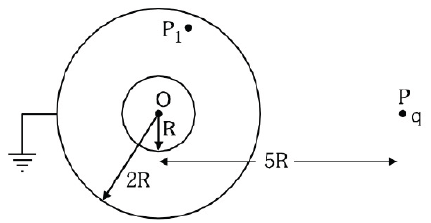
\includegraphics[width=0.7\linewidth]{Score-II - Test 42 (19 Mar 2025)-img/p1phy_q2_sphere.png}
\end{center}

\begin{qoptions}
\opt{A}{The modulus of charge on outer surface of solid sphere is $\dfrac{2Q}5$.}
\opt{B}{The electric field energy per unit volume at point P$_1$ is zero.}
\opt{C}{The magnitude of net electric force experienced by "q" due to charge on the sphere is $\left[\dfrac{2Kq^2}{125R^2}\right]$.}
\opt{D}{If the connection of sphere from ground is now removed then the potential energy of the system will increase.}
\end{qoptions}

\textbf{3.} As shown in the figure, balls 1 and 2 are both projected horizontally from the same point at a height H above the ground. Their horizontal initial velocities are v$_1$ and v$_2$ respectively, with v$_1>$v$_2$. Ball 1 is projected and barely clears the top of a vertical obstacle located at position x$_P$, and then falls on the ground at point R. The distance between point R and point O is R. After being projected, ball 2 falls to the ground and undergoes an elastic collision, then bounces back over the obstacle and lands again at point R.

\begin{center}
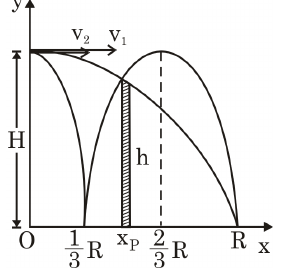
\includegraphics[width=0.55\linewidth]{Score-II - Test 42 (19 Mar 2025)-img/p1phy_q3_projectile.png}
\end{center}

\begin{qoptions}
\opt{A}{The ratio of $\dfrac{v_1}{v_2}$ is 2.}
\opt{B}{The position of obstacle x$_P$ is $\dfrac R2$.}
\opt{C}{The height of obstacle h is $\dfrac{3H}4$.}
\opt{D}{None of the above.}
\end{qoptions}

\textbf{4.} Intensity of x-rays coming from an x-ray tube is plotted against wavelength as shown:-

\begin{center}
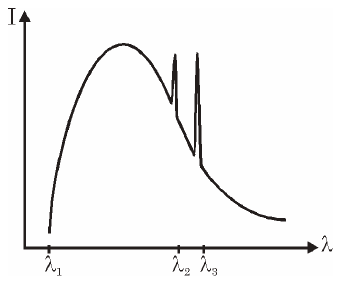
\includegraphics[width=0.75\linewidth]{Score-II - Test 42 (19 Mar 2025)-img/p1phy_q4_xray.png}
\end{center}

\begin{qoptions}
\opt{A}{If accelerating potential is changed, keeping target same, then sharp peaks ($\lambda_2$ \& $\lambda_3$) will shift to new positions.}
\opt{B}{If accelerating potential is changed keeping the target same, then minimum wavelength of spectrum ($\lambda_1$) will shift to new location.}
\opt{C}{In the radiation coming out of the tube, photons corresponding to wavelength $\lambda_3$ will have more energy than those corresponding to $\lambda_2$.}
\opt{D}{In the radiation coming out of the tube, number of photons corresponding to wavelength $\lambda_3$ will be more in number than number of photons corresponding to $\lambda_2$.}
\end{qoptions}

\textbf{5.} An electrical circuit consists of an ideal voltage source with an EMF $\varepsilon$, a resistor with resistance R, a switch, and a capacitor charged to a voltage of $\dfrac\varepsilon3$ (the polarity is indicated in the diagram). The capacitance of the capacitor is C. The resistance of the wires and the switch is negligible. The switch is closed.

\begin{center}
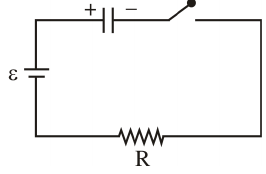
\includegraphics[width=0.55\linewidth]{Score-II - Test 42 (19 Mar 2025)-img/p1phy_q5_circuit.png}
\end{center}

\begin{qoptions}
\opt{A}{The maximum rate of change of energy in the capacitor is $\dfrac{\varepsilon_0^2}{4R}$.}
\opt{B}{The amount of heat released in this circuit by the time the maximum rate of change of the capacitor's energy is reached is $\dfrac5{72}C\varepsilon_0^2$.}
\opt{C}{The total amount of heat released in the resistor over a very long period of time after the switch is closed is $\dfrac29C\varepsilon_0^2$.}
\opt{D}{The total amount of heat released in the resistor over a very long period of time after the switch is closed is $\dfrac19C\varepsilon_0^2$.}
\end{qoptions}

\textbf{6.} Becquerel performed an experiment in which the particles emitted after radioactive decay were passed through a magnetic field. He measured magnetic rigidity which is a product of magnetic field and the radius of curvature $\rho$ of the particle in the magnetic field. The particles were emitted perpendicular to the magnetic field. Consider the reactions mentioned in options below. In each of the radioactive decay, a statement about the magnetic rigidity is made. Select the option(s) in which the statement correctly describes the outcome of the experiment.

\begin{center}
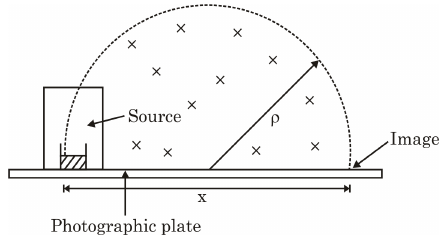
\includegraphics[width=0.85\linewidth]{Score-II - Test 42 (19 Mar 2025)-img/p1phy_q6_becquerel.png}
\end{center}
\emph{Figure: In Becquerel's arrangement $\beta$ rays from a radioactive source were deflected in a semicircular arc by a magnetic field into the plane of the paper}

\begin{qoptions}
\opt{A}{When $^{37}_{18}$Ar decays to $^{37}_{17}$C$\ell$, the radiation has magnetic rigidity which is found to vary from a certain non-zero minimum value to a certain maximum value}
\opt{B}{When $^{238}_{92}$U decays to $^{234}_{90}$Th, the radiation has magnetic rigidity which is the same for all the radiation}
\opt{C}{When $^{19}_8$O decays to $^{19}_9$F, the radiation has magnetic rigidity which is found to vary from zero to a certain maximum value}
\opt{D}{When $^{25}_{13}$A$\ell$ decays to $^{25}_{12}$Mg, the radiation has magnetic rigidity which is found to vary from zero to a certain maximum value}
\end{qoptions}

\subsectionhdr{Section-II: Numerical Value}

\textbf{1.} Shyam is sitting on a fixed bus seat with his feet off the floor. Here, he is modelled as 3 thin, rigid rods of uniform mass density joined to each other, with dimensions as shown in the figure. His seat consists of a base and a backrest. The coefficient of static friction between Shyam and the seat is $\mu=0.5$. The bus driver suddenly brakes at a constant deceleration and Shyam finds himself crashing into the seat in front of him. Fuming, Shyam decides to calculate the maximum bus deceleration a at which he would have remained stationary. What is the value of a (in m/s$^2$)?

\begin{center}
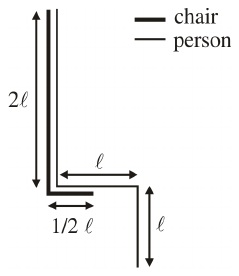
\includegraphics[width=0.75\linewidth]{Score-II - Test 42 (19 Mar 2025)-img/p1phy_n1_chair.png}
\end{center}

\textbf{2.} A uniform magnetic field of field strength B = 0.5 T runs parallel to the axis of a long insulating cylindrical shell of radius b = 35.0 m. A charged particle with mass m = 0.05 kg and charge q = 0.1 C is initially positioned at a distance a = 10.0 m away from the axis of the cylinder. The particle is launched with speed v = 25 m/s in an arbitrary direction. What is the minimum time taken t (in sec) for the particle to reach the wall of the cylinder?

\begin{center}
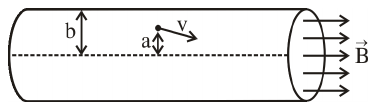
\includegraphics[width=0.85\linewidth]{Score-II - Test 42 (19 Mar 2025)-img/p1phy_n2_cylinder.png}
\end{center}

\textbf{3.} Ideal monatomic gas is contained within a sealed syringe. The piston in the syringe can be moved such that the volume can be varied between V and 4V. Simultaneously, valves in the syringe allow the pressure to be controlled between P and 2P. The gas starts out at pressure 2P and volume V. It is to be brought to final pressure P and volume 4V. Depending on how the piston and the valves are controlled over time, the heat absorbed by the gas in the process can range between Q$_{min}$ and Q$_{max}$. Find the ratio $\dfrac{Q_{max}}{Q_{min}}$. Assume that the piston and the valves are controlled such that the process undergone by the gas is reversible, and that the path traced by the process on the pressure-volume graph does not self-intersect.

\begin{center}
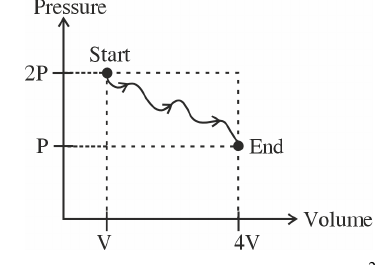
\includegraphics[width=0.75\linewidth]{Score-II - Test 42 (19 Mar 2025)-img/p1phy_n3_pvgraph.png}
\end{center}

\textbf{4.} There is 5 litres water at a temperature of 20$^\circ$C in a pot of base area 10 cm$^2$. The density of water is 998 kg/m$^3$. The water is heated to 80$^\circ$C. The coefficient of volume expansion of water can be considered constant between the temperature values of 20$^\circ$C and 80$^\circ$C, and it is $\beta_{\text{water}}=4\times10^{-4}$ K$^{-1}$. The pot is made of stainless steel whose coefficient of volume expansion is $\beta_{\text{steel}}=5\times10^{-5}$ K$^{-1}$. Neglect the vaporization of water. How much does the level of water change (in mm) due to the heating?

\textbf{5.} The lengths of the semi-major axis of two satellites orbiting around the Earth are the same. The ratio of the speeds of the two satellites when they are at perigee is 3/2, and the eccentricity of the orbit of that satellite which is faster at this point is 0.5. The eccentricity of the path of the other satellite is:-

\textbf{6.} Lamps with two different resistance values are connected as shown in the diagram. The circuit is connected to a voltage source, and the power dissipated in each of the lamps was found to be the same. The dependence of the lamp resistances on the current flowing through them can be neglected. Then, the lamp numbered 4 was swapped with the lamp numbered 1. The ratio $\dfrac{P_1}{P_2}$, where P$_1$ is the total power dissipated in the circuit initially, and P$_2$ is the total power dissipated in the circuit after swapping the lamps is

\begin{center}
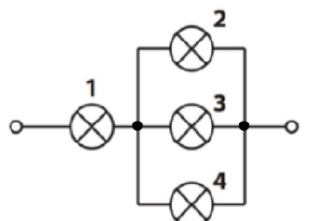
\includegraphics[width=0.65\linewidth]{Score-II - Test 42 (19 Mar 2025)-img/p1phy_n6_lamps.png}
\end{center}

\subsectionhdr{Section-III: Single Digit Integer}

\textbf{1.} A uniform solid spherical ball of radius r floats in water. The ball is displaced vertically downwards by a distance a $\ll$ r and released from rest, after which it oscillates with period T. After a long time t$_1\gg$T, its amplitude of oscillations drops below a fixed value $\delta\ll$a. If a ball of the same material and radius 2r is displaced by the same distance a, the time taken for its amplitude to drop below $\delta$ becomes t$_2$. Determine the ratio $\dfrac{t_2}{t_1}$. Assume that the damping force on the ball is given by Stokes' Law as F $=-6\pi r\eta v$; where $\eta$ is the viscosity of the water and v is the velocity of the ball.

\textbf{2.} Two masses 2 kg and 1 kg are attached to the ends of an inextensible long light string passing through a fixed smooth massless pulley as shown in the Figure. The masses are released when 2 kg is at a height h above the ground. The 2kg block comes to rest instantly after colliding with ground. It is found that during the time interval $\Delta t=\sqrt{\dfrac{nh}{3g}}$, the string remained tensionless. Find the value of n. [g-acceleration due to gravity].

\begin{center}
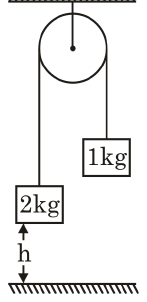
\includegraphics[width=0.35\linewidth]{Score-II - Test 42 (19 Mar 2025)-img/p1phy_n2b_pulley.png}
\end{center}

\textbf{3.} Monochromatic plane light with a wavelength of $\lambda=6000$ \r{A} is incident normally on the base of a thin prism with a small angle $\alpha$ and a refractive index n = 1.5. If the fringe spacing on the screen is 0.1 mm, find the prism base angle $\alpha$ (in radian). Fill the value of $1000\alpha$.

\begin{center}
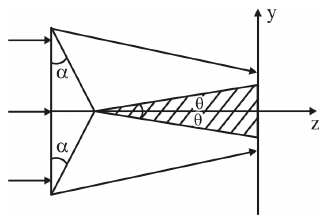
\includegraphics[width=0.75\linewidth]{Score-II - Test 42 (19 Mar 2025)-img/p1phy_n3_prism.png}
\end{center}

\textbf{4.} The following circuit consists of identical capacitors, each of capacitance C$_0$ = 22 $\mu$F. It's extremely wasteful, and Ram wishes to be prudent. Hence, he replaces this with a single capacitor of capacitance C$_{eq}$ between A and B. The value of $\left(\dfrac{C_{eq}}2\right)$ (in $\mu$F) is

\begin{center}
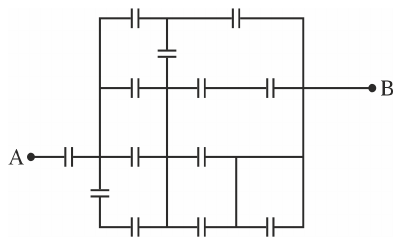
\includegraphics[width=0.75\linewidth]{Score-II - Test 42 (19 Mar 2025)-img/p1phy_n4_capnetwork.png}
\end{center}

\textbf{5.} In a long cylindrical metal wire of radius r and of resistivity $\rho$, a current of strength I flows in a uniform distribution. The wire has a constant surface temperature T$_0$. It is known that the metal has thermal conductivity k. The temperature difference (in K) between the axis of the wire and surface of the wire is:- (Take I = 4A, $\rho$ = 10 $\Omega$m, r = 10 cm, k = 100 W/m-k, $\pi^2$ = 10)

\textbf{6.} A thick spherical shell having density $2\sigma$ and outer radius R and inner radius r = $\dfrac R{(3)^{1/3}}$ is thrown downward inside a tank, containing a liquid having density $\sigma$. Value of rate of change of speed of the shell when the speed of the shell becomes v$_0=\dfrac{R^2\sigma g}{9\eta}$ (where $\eta$ is coefficient of viscosity and g is acceleration due to gravity) is g/k (m/s$^2$). Find the value of k.

\sectionhdr{PART-2: CHEMISTRY}
\subsectionhdr{Section-I: One or more correct}

\textbf{1.} The correct statement(s) for orthoboric acid is/are:

\begin{qoptions}
\opt{A}{when orthoboric acid is strongly heated, the residue left is boric anhydride}
\opt{B}{orthoboric acid does not act as a proton donor but acts as a Lewis acid by accepting hydroxyl ion.}
\opt{C}{orthoboric acid is obtained along with H$_2$ gas when diborane is hydrolysed}
\opt{D}{orthoboric acid is obtained by acidifying an aqueous solution of borax}
\end{qoptions}

\textbf{2.} If pH of an aqueous solution of 0.01M monoprotic acid HA is found to be 3 at T kelvin, then the correct information(s) is/are

\begin{qoptions}
\opt{A}{Degree of dissociation of the acid would be 10\%}
\opt{B}{Osmotic pressure of the solution would be 0.011RT}
\opt{C}{Theoretical molar mass of HA is 1.1 times of its observed molar mass}
\opt{D}{K$_b$ of A$^-$(aq.) is $10^{-4}$ (approx.) at 298K}
\end{qoptions}

\textbf{3.} Choose the correct statement(s) among the following regarding hydrogen atom? (All graphs given below are indicative in nature, not to scale)

\begin{qoptions}
\opt{A}{For an atomic orbital, radial wave function R(r) depends on principal, azimuthal and magnetic quantum number.}
\opt{B}{Plot of R$_{(2,0)}$(r) versus r (distance from nucleus), for 2s electron is \raisebox{-0.4\height}{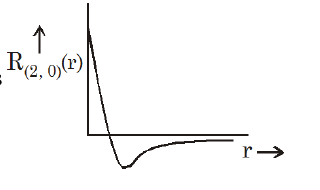
\includegraphics[width=0.42\linewidth]{Score-II - Test 42 (19 Mar 2025)-img/p2chem_q3B.png}}}
\opt{C}{Plot of R$^2_{(2.0)}$ versus r (distance from nucleus), for 2s electron is \raisebox{-0.4\height}{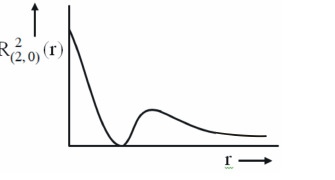
\includegraphics[width=0.42\linewidth]{Score-II - Test 42 (19 Mar 2025)-img/p2chem_q3C.png}}}
\opt{D}{Plot of $4\pi r^2R^2_{(2.0)}$ against r (distance from nucleus) is \raisebox{-0.4\height}{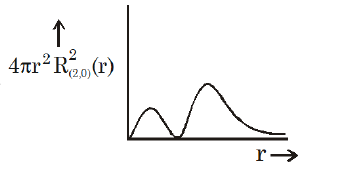
\includegraphics[width=0.42\linewidth]{Score-II - Test 42 (19 Mar 2025)-img/p2chem_q3D.png}}}
\end{qoptions}

\textbf{4.} Compound [Co(en)$_2$(NO$_2$)Cl]Br has:

\begin{qoptions}
\opt{A}{three ionisation isomeric form}
\opt{B}{two linkage isomeric form}
\opt{C}{two geometrical isomeric form}
\opt{D}{three stereoisomers}
\end{qoptions}

\textbf{5.} Which of the following amine(s) can not be prepared by Gabriel phthalimide reaction?

\begin{center}
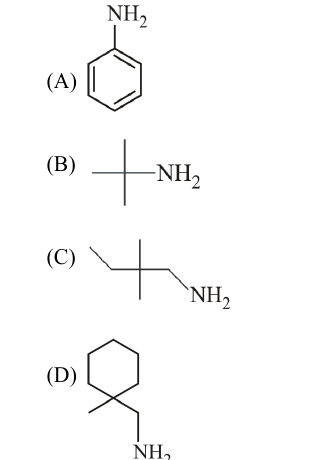
\includegraphics[width=0.35\linewidth]{Score-II - Test 42 (19 Mar 2025)-img/p2chem_q5_amines.png}
\end{center}

\textbf{6.} Choose the correct option(s) for the following set of reactions.

\begin{center}
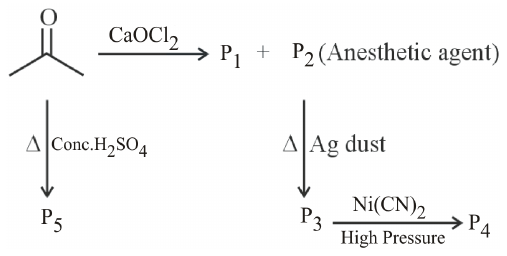
\includegraphics[width=0.85\linewidth]{Score-II - Test 42 (19 Mar 2025)-img/p2chem_q6_scheme.png}
\end{center}

\begin{qoptions}
\opt{A}{Conjugated $\pi$ electrons in product P$_4$ are 8}
\opt{B}{Product P$_4$ can undergo electrophilic addition reaction}
\opt{C}{Product P$_4$ is antiaromatic}
\opt{D}{Degree of unsaturation in product P$_5$ is 4}
\end{qoptions}

\subsectionhdr{Section-II: Numerical Value}

\textbf{1.} Total number of complex which diamagnetic and low spin in following complex compound. $[\text{Cr}(\text H_2\text O)_6]^{3+}$, $[\text{Co}(\text H_2\text O)_6]^{3+}$, $[\text{Ni}(\text{en})_3]^{2+}$, $[\text{HgI}_4]^{2-}$, $[\text{Cu}(\text{CN})_4]^{3-}$, $[\text{Fe}(\text{CN})_6]^{3-}$, $[\text{Co}(\text{ox})_3]^{3-}$, $[\text{NiF}_6]^{2-}$

\textbf{2.} 0.1 mole of white phosphorus reacts with 0.6 mole SOCl$_2$ to form a pungent smelling gas(A) alongwith other products. Gas(A) is reacted with 0.2 mole KMnO$_4$ in acidic medium and the product mixture is treated with excess BaCl$_2$ solution. A white precipitate insoluble in dilute acids is formed. Let the weight of precipitate formed be x gram. Find the value of $\dfrac x3$. (Molecular weight of Ba = 137)

\textbf{3.} Solid AgNO$_3$ is added to an aqueous solution containing 0.2 M Br$^-$ and 0.1 M I$^-$. Assuming that AgNO$_3$ addition does not change volume of this solution, calculate the percentage of [I$^-$] precipitated, when [Br$^-$] just starts precipitating: (Given: $k_{sp}$(AgBr) = $10^{-13}$ M$^2$; $k_{sp}$(AgI) = $10^{-17}$ M$^2$)

\textbf{4.} When an ideal gas having initial pressure P, volume V and temperature T, is allowed to expand adiabatically and reversibly until its volume becomes 5.66V, while its temperature falls to half. The workdone by the gas is represented by x times PV. Find the value of x. ($10^{0.3}=2$, $10^{0.48}=3$, $10^{0.75}=5.66$)

\textbf{5.} The number of resonating structures for organic compound P is

\begin{center}
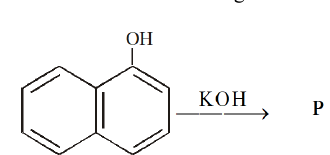
\includegraphics[width=0.55\linewidth]{Score-II - Test 42 (19 Mar 2025)-img/p2chem_n5_naphthol.png}
\end{center}

\textbf{6.} Number of geometrical isomers for product (U) is

\begin{center}
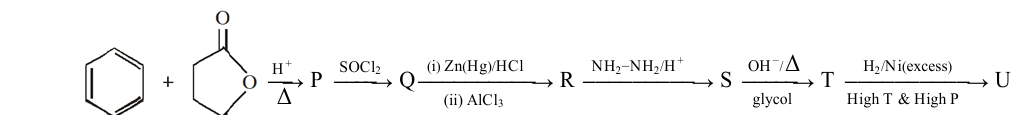
\includegraphics[width=0.95\linewidth]{Score-II - Test 42 (19 Mar 2025)-img/p2chem_n6_scheme.png}
\end{center}

\subsectionhdr{Section-III: Single Digit Integer}

\textbf{1.} A solution of weak acid HA was titrated with base NaOH. The equivalence point was reached when 50 mL of 0.1 M NaOH has been added. 25 mL of 0.1 M HCl was added to titrated solution and the pH was found to be 5.0. The pk$_a$ value of weak acid HA is \_\_\_\_\_.

\textbf{2.} For the complex compound [Pt(NH$_3$)(NO$_2$)py(ONO)], total number of geometrical isomers will be:

\textbf{3.} A list of species having the formula XZ$_4$ is given below: XeF$_4$, SF$_4$, SiF$_4$, BF$_4^-$, BrF$_4^-$, $[\text{Cu}(\text{NH}_3)_4]^{2+}$, $[\text{FeCl}_4]^{2-}$, $[\text{CoCl}_4]^{2-}$ and $[\text{PtCl}_4]^{2-}$. Defining shape on the basis of the location of X and Z atoms, the total number of species having a square planar shape is

\textbf{4.} Out of N$_2$O, SO$_2$, I$_3^+$, I$_3^-$, CN$_2^{2-}$, NO$_2^-$, N$_3^-$, C$_3^{4-}$, number of linear species is x, then find x:

\textbf{5.} Number of correct statement(s) is:

(i) Both D-Glucose \& D-Fructose give positive tollen's and fehling's test

(ii) D-Glucose \& D-Galactose form same osazone

(iii) Amylopectin is water insoluble while amylose is water soluble

(iv) Reaction of D-Glucose with HNO$_3$ yields Glucaric acid

(v) One mole of PhNHNH$_2$ reacts with 3 mol glucose to form osazone.

(vi) Reaction of D-Glucose with HI/Red P yields n-hexane

(vii) Vitamin B12 is a water soluble vitamin

(viii) Number of nitrogen atoms in one histidine molecule is 4

(ix) DNA is a polynucleoside

\textbf{6.} A (molecular formula C$_8$H$_{10}$O rotates PPL) reacts as follows: with Red P + HI it gives C (Optically inactive); with KMnO$_4$/H$^+$/$\Delta$ it gives B (C$_7$H$_6$O$_2$ molecular formula). A reacts with I$_2$ + NaOH to produce Yellow ppt. Also, (A) $\xrightarrow{\text{TsCl}}$ (D) $\xrightarrow[\text{KOH}/\Delta]{\text{alcoholic}}$ (E).

How many statement(s) are correct regarding the above set of reactions?

\begin{qoptions}
\opt{a}{(A) decolourises Br$_2$ water}
\opt{b}{(A) reacts with Na metal to give colourless odourless gas}
\opt{c}{(A) reacts with Lucas reagent to give turbidity after 5-10 minutes}
\opt{d}{(B) is \raisebox{-0.35\height}{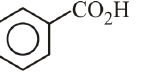
\includegraphics[width=0.32\linewidth]{Score-II - Test 42 (19 Mar 2025)-img/p2chem_n6_optD_benzoic.png}}}
\opt{e}{(C) does not react with NBS/h$\nu$}
\opt{f}{(D) is optically active and can undergo S$_N$2 reaction}
\opt{g}{(E) decolourises Br$_2$/H$_2$O solution}
\opt{h}{(E) can undergo electrophilic addition reaction as well as electrophilic aromatic substitution reaction}
\opt{i}{(E) can undergo addition polymerisation reaction}
\end{qoptions}

\sectionhdr{PART-3: MATHEMATICS}
\subsectionhdr{Section-I: One or more correct}

\textbf{1.} Let n be a positive integer with $f(n)=1!+2!+3!+\ldots.n!$ and g(x) and h(x) are polynomials such that $f(n+2)=g(n)f(n+1)+h(n)f(n)\ \forall\ n\ge1$, then which of the following is/are correct

\begin{qoptions}
\opt{A}{g(100) = 103}
\opt{B}{h(48) = $-50$}
\opt{C}{g(50) = 52}
\opt{D}{h(42) = $-43$}
\end{qoptions}

\textbf{2.} Let $\left(1+\dfrac1n\right)^{n+x_n}=e$ and $\displaystyle\lim_{n\to\infty}x_n=k$
$$f(x)=\sum_{r=1}^m\left(x^r+x^{-r}\right)^{1/k},\ x\ne\pm1$$
$$\resizebox{\linewidth}{!}{$g(x)=\begin{cases}\displaystyle\lim_{m\to\infty}(f(x)-2m)x^{-2m-2}\cdot(1-x^2), & x\ne1,-1,0\\[4pt] -1 & \text{for }x=\pm1\end{cases}$}$$
then g(x) is:

\begin{qoptions}
\opt{A}{discontinuous at x = $-1$}
\opt{B}{continuous at x = 2}
\opt{C}{limit exist at x = 1}
\opt{D}{limit does not exist at x = 1}
\end{qoptions}

\textbf{3.} $\displaystyle\int\cos^{2n+1}x\,dx=\dfrac{\sin x}{a_1}-{}^n C_1\dfrac{\sin^3x}{a_2}+{}^nC_2\dfrac{\sin^5x}{a_3}-\ldots\ldots\ldots+(-1)^n\dfrac{\sin^{2n+1}x}{a_n}+c$ (where C is the constant of integration)

If $a_1+a_2+a_3+\ldots..+a_n=\lambda(n+1)^2$ and $\displaystyle\int\dfrac{dx}{(x^3+\lambda)^2}=A\displaystyle\int\dfrac{dx}{(x^3+\lambda)}+\dfrac{Bx}{x^3+\lambda}$

\begin{qoptions}
\opt{A}{A + B = $\lambda$}
\opt{B}{A $-$ B = $\dfrac13$}
\opt{C}{A + 2B = $\dfrac43$}
\opt{D}{A = 2B = $\dfrac\lambda3$}
\end{qoptions}

\textbf{4.} Let $f(k)=\displaystyle\sum_{r=1}^k\dfrac1r$ and $\displaystyle\sum_{r=1}^{2023}f(r)=af(b)+c$ and b = 2023, a,c$\in$I then which of the following is/are true

\begin{qoptions}
\opt{A}{b = c}
\opt{B}{a $-$ b = 1}
\opt{C}{b + c = 0}
\opt{D}{a + c = 0}
\end{qoptions}

\textbf{5.} Given that number of solution of the equation $\dfrac15\log_2x=\sin5\pi x$ is N then N is

\begin{qoptions}
\opt{A}{divisible by 3}
\opt{B}{perfect square}
\opt{C}{greater than 121}
\opt{D}{less than 155}
\end{qoptions}

\textbf{6.} Let a$_i$, i = 1,2,3,\ldots,n denote integers in the domain of $f(x)=\sqrt{\log_{1/2}\left(\dfrac{4x-25}{x-21}\right)}$ where a$_i<$a$_{i+1}\ \forall i\in\mathbb N$. If line L: $\dfrac{2x-a_1}4=\dfrac{y+a_1}{a_2}=\dfrac{z-z_3}{a_5}$ meets xy, yz, zx planes at A, B, C respectively and D is image of C in x axis then volume of tetrahedron OABD is V, where O is origin and $\Delta_1,\Delta_2,\Delta_3,\Delta_4$ are areas of faces and h$_1$, h$_2$, h$_3$, h$_4$ corresponding altitudes of any tetrahedron PQRS. (In case PQRS is regular tetrahedron, volume of PQRS is equal to volume of OABD). Assuming minimum value of $\displaystyle\sum_{1\le i\ne j\le4}\sum\Delta_ih_j$ is $\lambda$, then which of the following is/are true

\begin{qoptions}
\opt{A}{$\lambda+9V=140$}
\opt{B}{$\lambda-40[V]=8$ ([.] is greatest integer function)}
\opt{C}{sum of digit of 9V is 10}
\opt{D}{sum of digits of $\lambda$ is 4}
\end{qoptions}

\subsectionhdr{Section-II: Numerical Value}

\textbf{1.} If number of positive terms in the sequence $a_n=\dfrac{195}{4\ ^nP_n}-\dfrac{^{n+3}P_3}{^{n+1}P_{n+1}}$, $n\in\mathbb N$ is a and $b_1+b_3+b_5+b_7+b_9+b_{11}+b_{13}=b$ where b$_k$ is digit in the units place of number $(1!+2!+\ldots.+k!)$, $k\in\mathbb N$, then $\dfrac ba$ equals

\textbf{2.} If the locus of middle point of contact of tangent drawn to the parabola $y^2=8x$ and the foot of perpendicular drawn from its focus to the tangent is a conic then find latus rectum of the conic.

\textbf{3.} Three circles with radius 3 have centres at P(14, 92), Q(17, 76) and R(19, 84). A line passes through Q such that total area of the parts of the three circles to one side of the line is equal to the total area of the part of three circle to the other side of it. If slope of line is m then $\dfrac{|m|}5$ is equal to

\textbf{4.} Let real number x, y, z, w satisfy $\dfrac{x^2}{n^2-1}+\dfrac{y^2}{n^2-3^2}+\dfrac{z^2}{n^2-5^2}+\dfrac{w^2}{n^2-7^2}=1$ for n = 2, 4, 6, 8. Value of $\dfrac{x^2+y^2+z^2+w^2}{10}$ equals

\textbf{5.} $N=\left[\displaystyle\sum\log_{10}K\right]$ where [.] greatest integer function and $\sum$ denotes summation of all values of $\log_{10}k$ where k is positive divisor of 1000,000 excluding $10^6$ itself. Then $\dfrac N{100}$ is

\textbf{6.} There are `m' red socks and `n' blue socks in a bag. Where m + n $\le$ 1991. Let two socks taken out at random, probability that they have the same colour is $\dfrac12$. If largest possible value of m is P then $\left(\dfrac{1000-P}8\right)$ equals

\subsectionhdr{Section-III: Single Digit Integer}

\textbf{1.} The equation $\sec\theta+\text{cosec}\theta=c$ has two solutions between 0 and $2\pi$ if $c^2<k$ and four solutions if $c^2>k$. Find number of integral solution of the equation $x^2+k+6x=0$

\textbf{2.} Let matrix $A=\begin{bmatrix}3&2\\1&1\end{bmatrix}$ satisfies the equation $A^2+aA+bI_2=0$ and value $\displaystyle\int_a^{4b}x^3\cos x\,dx=\dfrac{ma+nb}{na-mb}$. (where m, n are least positive integers). Evaluate the sum of diagonal elements of the matrix $\begin{bmatrix}m+n-1&m^2n^2\\-m&-n\end{bmatrix}^{2025}$. (where I$_2$ is an identity matrix of order = 2)

\textbf{3.} E$_1$ and E$_2$ are two ellipses such that area of ellipse E$_2$ is one third of the area of quadrilateral formed by tangents at the ends of latus rectum of the ellipse E$_3\equiv5x^2+9y^2=45$. E$_1$ is inscribed in E$_2$ in such a way that both E$_1$ and E$_2$ touch each other at one end of their common major axis. Given length of major axis of E$_1$ equals length of minor axis of E$_2$ and eccentricities of E$_1$, E$_2$, E$_3$ are equal then the area of E$_2$ lying outside E$_1$ equals

\textbf{4.} If $f:\mathbb R-\{-1\}\to\mathbb R$, f(x) is a differentiable non-constant, non-identity function satisfies, $f(x+f(y)+xf(y))=y+f(x)+yf(x)\ \forall\ x,y\in\mathbb R-\{-1\}$, then $2025(1+f(2024))$ equals

\textbf{5.} Let x, y, z, w are non-zero complex numbers such that $w=x^{24}=y^{40}=x^{12}y^{12}z^{12}$, if z = 1 + i find the remainder when $|w|$ divided by 7 is

\textbf{6.} Let $x^2+bx+6b=0$ has only integer roots. If number of real values of `b', is n then value of $\dfrac n2$ equals

\end{multicols}
\end{document}
